\documentclass{bioinfo}

\usepackage{scrextend}
\usepackage{fullpage} 
\usepackage{parskip} 
\usepackage{tikz} 
\usepackage{amsmath}
\usepackage{float}
\usepackage{graphicx}
\usepackage{caption}
\usepackage{subcaption}
\usepackage[font=footnotesize, labelfont={sf,bf}]{caption}


\copyrightyear{2016}
\pubyear{2016}

\begin{document}
\firstpage{1}

\title[Project Proposal]{\Large{Modeling Heterogeneity in Microbial Population Dynamics}}
\author[Helena Herrmann]{Helena Herrmann$^{1}$}
\address{$^{1}$School of Computing Science, Newcastle University, UK}

\history{MSc Computational Systems Biology\\
Project Proposal for 14/04/2016 \\
Word Count: 3620} %Remember to update word count at the very end 
\vspace{-3em}
\editor{\normalsize{Supervision by Dr Conor Lawless, Institute for Cell and Molecular Sciences, Newcastle University, UK}}
\maketitle

\section{Introduction}

Cell growth rate is an important component of evolutionary fitness and is thus subjected to great selective forces; a reduced growth rate is generally strongly indicative of a struggling strain. Hence growth rate, a measure of how quickly cells are progressing through the cell cycle, can be considered a key cell phenotype. One way of measuring growth rate is through modeling. When capturing cell population dynamics through modeling the growth rate parameter is typically measured at the population scale; a scale chosen for technical convenience. 

Population scale measurements generally assume that observat- ions are directly transferable to the single cell level. However, there is increasing evidence that, even among isogenic populations, there is considerable heterogeneity in growth rates (e.g. \citealp{Pin06}; \citealp{Schmidt12}; \citealp{Levy12}). The idea of phenotypic heterogeneity arising through non-genetic differences (e.g. epigenetics (\citealp{Bird07}), cell age (\citealp{Ginovart11}), or selection pressure (\citealp{Navin11})) is beginning to receive much needed attention as it finds applications in modeling the dynamics of microbial infections, food security assessments, and tumorigenesis dynamics, to name a few.  For example, understanding the dynamics underlying isogenic, heterogeneous cell lineages has been marked as a key requirement for developing more effective cures in cancer research (\citealp{Tabassum15}). Our proposed work in yeast may very well provide a tractable model for such investigations. 

This project aims to address the extent to which models are able to accurately capture observable levels of growth rate heterogeneity from single isogenic microbial growth curves and to explore how this inter-cellular variability affects our interpretations of population growth rate. While cell growth is generally thought to go through four well-known phases (Figure~\ref{fig:GrowthPhases}), we would like to assess how these population level observations differ from those at the single lineage level. This project will concern itself with the lag phase and the exponential phase, where observed growth rates are most variable and have the greatest impact on apparent lineage fitness. 

We will develop models to capture observable levels of growth rate heterogeneity in isogenic microbial cultures. Novelty will arise from the fact that individual cells lineages will be analyzed separately, which will allow for us to explore inherent heterogeneities. We will then use the developed models to explore how intra-cellular variability can affect our interpretation of population growth rate observations.

\vspace{+2em}
\begin{figure}[H]
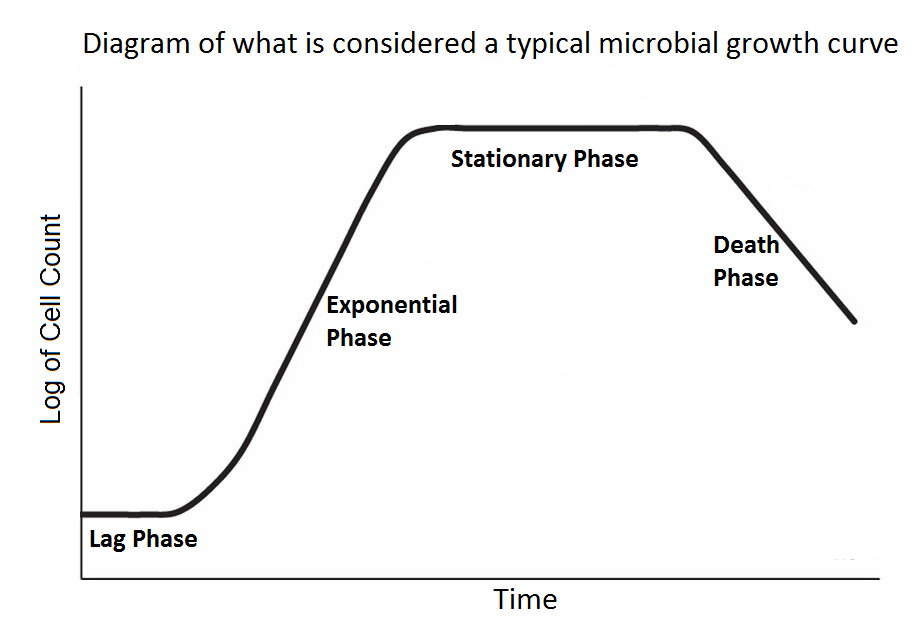
\includegraphics[width=1\linewidth]{GrowthPhases.png}
\caption{Diagram of microbial growth phases: (i) lag phase, where inoculated cells adapt to their new environment, (ii) exponential growth phase, where cells divide at a constant growth rate, (iii) growth arrest phase, where system carrying capacity is reached (iv) and death phase, where viable cell counts are declining. The described phases of growth are typically observed at the population level and are often also assumed to apply at the individual cell level (\citealp{Baranyi02}).}
\label{fig:GrowthPhases}
\vspace{-3em}
\end{figure}

We hypothesize that when accounting for intrinsic variation in cell division time and growth rate, new mechanistic insights will be gained, since the apparent heterogeneity between populations may be drastically reduced when considering single lineage heterogeneities. In particular, we will address the lag phase, as this is physiologically and mathematically the least explored growth phase as of today (\citealp{Rolfe12}). We hope to demonstrate that due to inter-lineage variability in growth rate, single lineage and population level observations differ. 

\section{Aims}

\textbf{1. Find a model which best captures heterogeneity in microbial growth curves through single lineage observations.}
\begin{addmargin}[1.5em]{1.5em}
This is based on the notion that isogenic cell growth exhibits intrinsic stochasticities which may drown in the noise of extrinsic heterogeneities when considering population dynamics. Addressing the effect of isogenic variation on cell lineage dynamics may yield further mechanistic insight for analyzing population growth curves. Can we find a stochastic model which reduces the apparent heterogeneity in growth rates in the data?
\end{addmargin}

\textbf{2. Explore the implications which single lineage modeling may have on the interpretation of various growth phases.} 
\begin{addmargin}[1.5em]{1.5em}
$\mu$QFA video data obtained by Lawless provides little evidence for a lag phase at first sight (\citealp{Lawless13}). It is suspected that when taking cell growth and division time into account, the lag phase may actually be a mere artifact of a wide growth rate distribution as shown for the two strains in Figure~\ref{fig:GrowthRateDistr}, as  well as the fact that fitter strains will become more densely distributed over time as a result of selection. Can explicit modeling of cell lineages give rise to an apparent lag phase at the population level even though this may not be visible at the single cell level? 

Additionally, microbiologists often sample cell populat- ions during the exponential phase in order to improve the reproducibility as fitter lineages are likely to be dominating the population at this point. It is thus worth analyzing how apparent population heterogeneity affects sampling from different phases.
\end{addmargin}

%\vspace{-1em}
\begin{figure}[H]
\centering
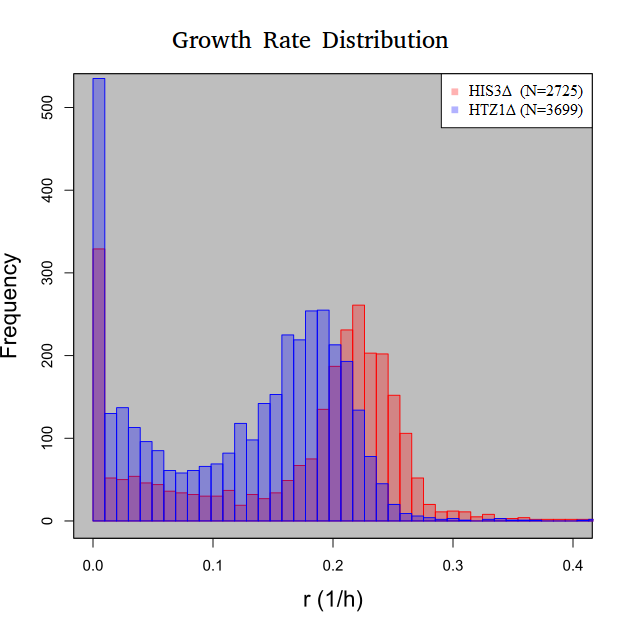
\includegraphics[width=0.8\linewidth]{GrowthRateDistr.png}
\caption{Growth rate distributions measured in wild-type \textit{his3}$\Delta$ and a sicker \textit{htz1}$\Delta$ strain using novel $\mu$QFA method.}
\label{fig:GrowthRateDistr}
\vspace{-2em}
\end{figure}

\textbf{3. Depending on resource availability and findings, repeat the micro Quantitative Fitness Analysis ($\mu$QFA) experiments with the aim of validating model predictions.}
\begin{addmargin}[1.5em]{1.5em}
This will involve undertaking microscopic observations of clonal \textit{Saccharomyces cerevisiae} cells to capture the lag and exponential phase of growth in great detail. Existing in-house image analysis software will be used for generating growth curves from the data, where the measured area of clonal cell cultures translates to the total number of cells at a given time. Following an iterative systems biology protocol, this step would allow us to grow cells at a higher or lower density than the current data, in order to test the predictions and generality of our models. 
\end{addmargin}

\vspace{-1.5em}
\begin{figure}[H]
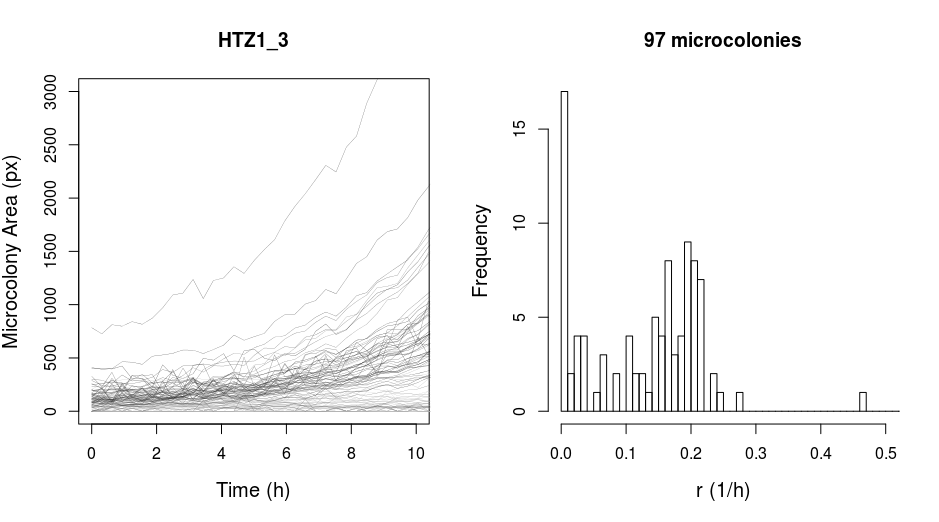
\includegraphics[width=1\linewidth]{LawlessExampleOutput4.png}
\end{figure}
\vspace{-4.3em}
\begin{figure}[H]
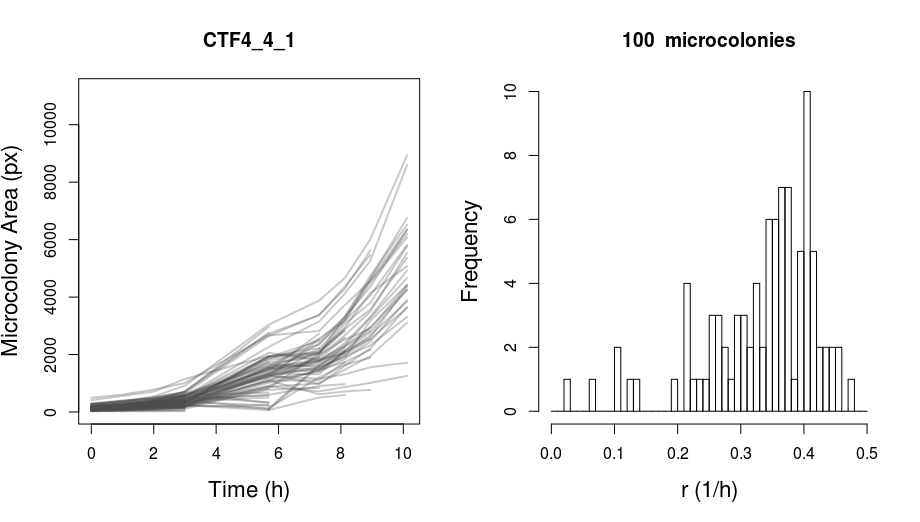
\includegraphics[width=1\linewidth]{LevyExampleOutput.png}
\end{figure}
\vspace{-4.3em}
\begin{figure}[H]
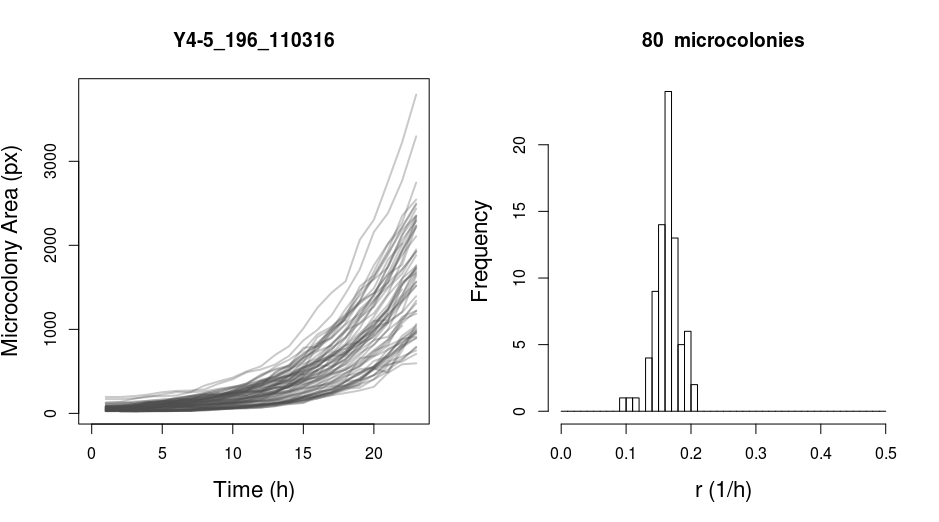
\includegraphics[width=1\linewidth]{ZivExampleOutput3.png}
\caption{Example outputs of clonal colony growth curves and the associated growth rate frequencies generated from each of the three data sets: Lawless (top), \citealp{Levy12} (middle) and \citealp{Ziv13} (bottom). Growth rates were estimated using the \texttt{lm} linear regression function in R, whereby the growth rate is equal to the slope of log(area) $\sim$ time.}
\label{fig:ExampleOutput}
\end{figure}
%\vspace{-1em}

\section{Proposed Research}

\subsection{Obtained Data}

To capture growth rate heterogeneity, we will develop a range of models and test their validity against available data. In order to ensure that our analysis holds under a range of experimental conditions and genetic backgrounds, we will explore three data sets: (i) $\mu$QFA data produced by Lawless (unpublished), (ii) high-throughput microscopy assay data produced by \citealp{Levy12} and (iii) \citealp{Ziv13}. All data sets consist of \textit{S. cerevisiae} micro-colony growth curves.

Clonal cultures are lineages derived from a single cell. Population pooling examines purified cell populations in order to learn about the behavior of single cells, thereby assuming that all members of the population behave in the same way. However, as shown in Figure~\ref{fig:ExampleOutput}, which displays growth curves obtained from clonal cultures grown in the same microplate well, this assumption seems rather far fetched. Figure~\ref{fig:ExampleOutput} shows that all three of the above data sets provide evidence for existing heterogeneities within clonal cultures, none of which has been detailed in a publication at the single lineage level. We propose to split the starting population up into individual cells and treat them as separate experiments. This will allow us to examine inherent stochasticities, which would otherwise drown in population noise. 

\subsection{Types of Models}

We propose to explore different types of models, including a logistic, deterministic model (\citealp{Verhulst45}), a standard Gillespie, birth-only stochastic model (\citealp{Bailey64}; \citealp{Gillespie77}), and a hybrid model which will combine the previous two models. Model implementations will be done in R and Python and should be relatively straightforward. 

A traditional, deterministic, logistic population growth model will be taken into consideration for its computational speed, which will be of a great advantage considering our vast amount of available data.

\vspace{-1em}
\begin{figure}[H]
\centering
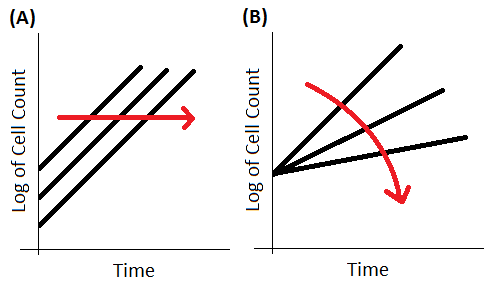
\includegraphics[width=0.7\linewidth]{HeterogeneityTypes.png}
\caption{Types of heterogeneity in the exponential phase which may arise between growth curves as indicated by the red arrows: (A) heterogeneity arising from a difference in starting population at the beginning of the exponential phase, and (B) heterogeneity arising from a difference in growth rate.}
\label{fig:HeteroTypes}
\vspace{-2em}
\end{figure}

However, as we would like to include cell lineage intrinsic growth-rate heterogeneities these will have to be captured using a stochastic model. A deterministic model will only be able to capture exponential growth heterogeneities arising from differences in the onset of the exponential phase as illustrated in Figure~\ref{fig:HeteroTypes} (A), whereas a stochastic model will additionally be able to capture inter-lineage growth rate heterogeneities, as sketched in Figures~\ref{fig:HeteroTypes}  (B). Thus, being able to compare stochastic and deterministic modeling may lead us to further conclude where the greatest heterogeneities lie within in the data and how these affect population level observations. Much of the theoretical ground work for stochastic growth models has been laid by Baranyi (1997, 1998, 2002); however, its application to high-throughput microbial sets of increased precision, which have become available since, remains limited. 

\subsection{Generating Biologically Meaningful Models}

Since the experimentally observed growth of microbial colonies (and, incidentally, that of human fibroblast populations) occurs in a monotonically increasing fashion during the lag and exponential phase, we will make use of birth-only models, deviating from more traditional birth and death conflict analyses. As far as we are aware, this will be the first time that birth-only models will be considered in the context of stochastic cell growth. 

Furthermore, it may prove sensible to set a lower bound for the time sampling step in the stochastic algorithm (deviating from the original Gillespie algorithm; \citealp{Gillespie77}). Doing so will allow us to incorporate the expected time required for cell growth and division, as an infinitesimal  growth and division time holds little biological meaning in the context of cell growth. 

Although we generally propose for our models to follow a birth-only process (\citealp{Bailey64}), it may also be of interest to see whether there is a low rate of death which can still give rise to monotonically increasing growth curves at the population level and whether this should be incorporated into the model. Alternatively it may be worth incorporating a transition to a non-dividing state, whereby cells remain in the population but cell division is suspended. For example, inocula suspected to be non-dividing cells which remain part of the population as observed in the $\mu$QFA data have been circled  red in Figure~\ref{fig:NonDividingCells} and are further confirmed by referring back to Figure~\ref{fig:GrowthRateDistr} where the majority of cells exhibit a growth rate between 0 $h^{-1}$ and 0.1 $h^{-1}$. 
%Here, selection pressure analyses or replicative-age measured in bud scars may provide further insights.

Lastly, in order to outweigh the computational cost associated with a stochastic model, a hybrid model combining the two approaches is also proposed to be validated against the data. For example, we may find that most of the inter-lineage variability arises early on in cell growth and thus we begin with a stochastic model, but that after a few initial divisions, growth curves closely follow a deterministic model, at which point it may seem sensible to induce a model switch. 

\begin{figure*}[ht!]
\centering
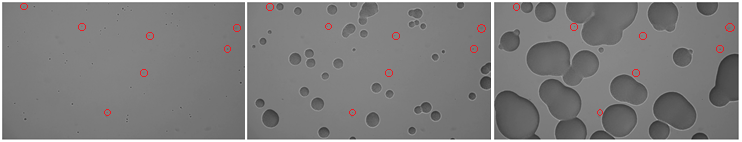
\includegraphics[width=1\linewidth]{NonDividing3Pics.png}
\caption{Colony growth based on the $\mu$QFA data after inoculation (left), after $\sim 1$ hour (center) and after $\sim 10$ hours (right), where non-growing inocula (suspected non-dividing cells) have been circled in red.}
\label{fig:NonDividingCells}
\vspace{-2.5em}
\end{figure*}

\subsection{Parameter Inference}

We will explore likelihood-free parameter inference techniques in order to obtain the required parameters from each of the data sets. Various options such as \verb pyMC \ for deterministic modeling, or the particle MCMC described by \citealp{Wilkinson06}, for stochastic modeling, are available foundations to work off. 
% To obtain the growth rate and carrying capacity parameters from each data sets we will follow the particle Markov chain Monte Carlo (MCMC) inference approach described by \citealp{Wilkinson06}, as this circumvents analytic evaluations of the likelihood functions. The starting population will be assumed as obtained from area to cell count calibrations; and uninformative priors are considered sufficient. Because the MCMC output, i.e. the posterior distribution, is not independent, we will accommodate for this via thinning (e.g. 100,000 updates with a burn-in of 100). 
Workflows for parameter inference will be documented for ease of model development. Evidently, only a subset of the available data can be used for parameter inference, as the rest will be required for model testing. Due to the huge amount of data at our disposition we can safely consider using up to half of the data from each of the sets (e.g. 3 out of 6 replicates) to train the models, as this will leave us with plenty of growth curves to validate the model against. 

Because we also have, from previous research done at Newcastle University, access to a full QFA data set (\citealp{Addinall11}), we can use all of the available microcolony growth curves from the $\mu$QFA data to obtain the models. We can then use these models to simulate a QFA population growth curve and compare our prediction (based on the single lineage $\mu$QFA data) with the population QFA observations. This will have the added advantage of showing the distinction between single lineage averages and observed population growth rates driven by selection. 

\vspace{-1em}
\subsection{Model Fit}

Finalized models will be validated using either the Bayesian Information Criterion (BIC) (\citealp{Schwarz78}) or Bayes factors (\citealp{Kass95}). \citealp{Christensen11}, provide a useful introduction to both model comparison techniques. Both the BIC and Bayes factors select from a range of models the one which corresponds to the greatest posterior probability, the difference lying in that the BIC does not require explicitly specified priors whereas Bayes factors do (\citealp{Bollen12}). An appropriate comparison technique will thus have to be chosen based on how confident we will be in establishing prior distributions. Notably, although very similar in implementation, the BIC would always be chosen over the Akaike Information Criterion (AIC) as it penalizes over-fitting more stringently (\citealp{Burnham02}), which will prove valuable when considering models with additional biological parameters as described above. As always, following a Bayesian paradigm over a frequentist one not only incorporates estimation uncertainty but also parameter uncertainty (\citealp{Christensen11}). The model with the best fit will then be used to explore the mechanistic implications of microbial cell growth. 

% Following the Bayesian paradigm, this model comparison technique selects from a range of models the one which corresponds to the greatest posterior probability, as indicated by its minimum BIC (\citealp{Schwarz78}). This methodology is chosen over that of computing a Bayes factors, as it does not require explicitly specified priors, instead using empirical log-likelihoods; yet the BIC remains roughly equivalent to the theoretical precision of Bayes factor (\citealp{Kass95}; \citealp{Bollen12}). 

\begin{figure*}[hb!]
\vspace{-1em}
\centering
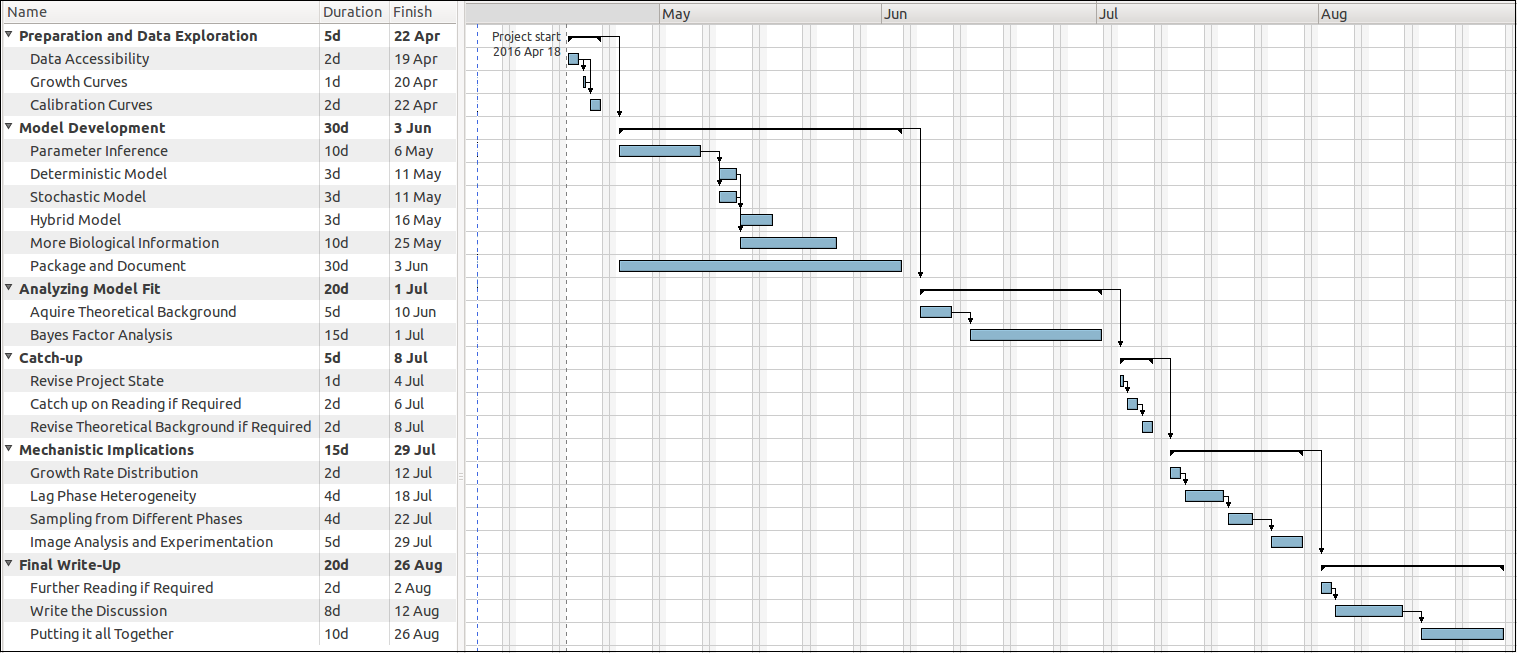
\includegraphics[width=1\linewidth]{GanttChart.png}
\caption{Gantt chart for the above outline objectives for completing the MSc Dissertation by August 26th, 2016.}
\label{fig:GanttChart}
\vspace{-0.5em}
\end{figure*}

\vspace{-1em}
\subsection{Model Predictions and Mechanistic Implications}

Upon parameter realization and model validation we can begin to analyze the mechanistic implications. Additionally, it may prove valuable to return to the lab in order test our model predictions. We have at disposition some \textit{ibidi} microscopy slides (16 well), which can be used for generating microbial growth curves. For the $\mu$QFA experimental design, please refer to \citealp{Lawless12}. 

As for the lag phase, there currently exists no explicit definition in the literature. Divergent definitions either define the lag phase to occur before the first cell division (\citealp{Baty04}) or to last over multiple cell divisions during which exponential growth has not yet begun (\citealp{Pin06}). \citealp{Rolfe12} are one of the only research groups that define (yet do not act upon) this distinction, using the terms \textit{lag phase} and \textit{delay phase}. These discrepancies can be even further subdivided in that some texts within the existing literature consider a biological definition of the lag phase (time until maximum growth acceleration; \citealp{Buchanan90}) or a mathematical definition (time until the tangent to the growth curve intersects that of the exponential growth phase; \citealp{Baranyi02}). 
%Furthermore, while it has generally been assumed that exponential growth begins after the first cell division (\citealp{Baty04}), \citealp{Pin06}, used \textit{Escherichia coli} single-lineage cell divisions to show that exponential growth begins only after the third or fourth cell division.

We on the other hand hypothesize that the lag phase itself may not be visible in single lineages, but arises as an artifact of intrinsic noise at the population level. It is suspected that when using stochastic modeling to reduce the apparent heterogeneity in the data, the lag phase is merely the result of a wide growth rate distribution. Correlations between a short lag phase and yeast cell age (negative correlation) and a short lag phase and inoculum size (positive correlation) exist, implying that cell growth and cell division can indeed occur almost immediately after inoculation (\citealp{Ginovart11}). Because the  $\mu$QFA data by Lawless provides very little evidence for a lag phase \textit{per se} (\citealp{Lawless13}), we hope to demonstrate that the lag phase can be apparent at the population level, despite being absent at the single lineage level. In the $\mu$QFA data, cells divide almost immediately, with some clones dividing more quickly than others. Thus we hypothesize that the lag phase arises at the population level as a result of inter-lineage variability in growth rate which arises as a result of competition between clonal cell lineages. It may very well be that as a result of competition, we observe a wide range of growth rates, which in turn results in very noisy population observations. 
%We expect that the explicit modeling of cell lineages may give rise to an apparent lag phase at the population level, but not at a single-lineage level.  
% By incorporating the time required for cell growth and division as a lower bound for time sampling along with the high resolution data, we hope to demonstrate that the lag phase can be apparent at the population level, despite being completely absent at the single cell level, due to inter-lineage variability in growth rate. We hypothesize that the explicit modeling of cell lineages may give rise to an apparent lag phase at the population level, but not at a single-lineage level. 

A second mechanistic implication worth our attention lies in the standard practice of micro-biologists to sample cell populations from dynamic growth phases rather than stationary ones in order to improve the reproducibility of their results. Given the dynamic aspect of cell growth it would be false to conclude for the maximum likelihood estimator of the initial growth rate distribution to apply over time. This is due to the fact that weaker strains (i.e. those with a reduced growth rate) are slower at producing offspring; thus, after a given amount of time the population will be dominated by faster growing strains. This is a likely explanation for why it has been noted that samples later on during the time course (i.e. the exponential phase) are more reproducible. However, sampling from the exponential phase again assumes members of the population to behave in the same way. Looking at single cell lineages as we propose will enable us to explore the implications of sampling at different growth phases and thus analyze the validity of experimental design procedures. 

\vspace{-1em}
\section{Objectives}
The above proposed research has been summarized in work packages shown below. The outlined objectives provide a step-by-step guidance for project advancement. All workflows will be documented and all models will be packaged to maximize accessibility, reproducibility and impact in the wider research community. 

Model packaging will occur during the development stage so that finalized models are used for the analysis steps. Dissertation write-up will occur throughout the project in the form of blog posts, whereby each stage as outlined in the objectives is to be completed before moving on to the next one. A full time-line for each of the objectives is provided; Figure~\ref{fig:GanttChart} displays a Gantt chart following these objectives. Time assigned for task completion is mostly generous as this project allows for much refinement and addition of detail should there be time (e.g. testing models with more biological information and obtaining further experimental data). One week for catching-up is scheduled in to account for unexpected difficulties, should these arise.

\vspace{-1.5em}
\begin{enumerate}
\item \textbf{Preparation and Data Exploration}
	\begin{enumerate}
    \item Ensure data accessibility by converting all three data sets into a general format which can be accessed using R and Python.
    \item Write scripts to extract growth curves from each of the data sets. Look at pulling out single growth curves and pulling out all growth curves for a single spot or genotype. 
    \item Use calibration curves to convert area vs. time curves to cell count vs. time curves. 
    \end{enumerate}
    
\textit{Write up: Stage 1 – Introduction and Background Reading (reuse project proposal). Generate plots to visualise the raw data for why the impact of heterogeneity is being researched.} \\

\item \textbf{Model Development}
	\begin{enumerate}
    \item Develop parameter inference workflows to learn about microbial growth rates. 
    \item Fit a deterministic model to all data using a Bayesian hierarchical model in \verb pyMC  using a subset of the available data.  
    \item Fit a stochastic birth-only model to a subset of the available data. 
    \item Fit a hybrid model to to a subset of the available data. Can a sensible cut-off for model switching be determined? 
    \item Remaining data can then be used to explore heterogeneity; for example, the HIS3$\Delta$ and the HTZ1$\Delta$ strains are considered in all three data sets. Consider comparing $\mu$QFA and QFA data.
    \item Can we improve the models by adding more biological information? Consider using the time required for cell growth and division as a lower bound for time sampling in the algorithm of the stochastic model. Potentially consider more complicated models which include some kind of death, or alternatively a switch to a non-dividing state, while maintaining monotonic increasing growth curves. Is there a low rate of death which can still give increasing curves?
    \item Package and document the models.
    \end{enumerate}

\textit{Write up: Stage 2 - Model development. State model assumptions, implications, and validity. Analyze how these model fits differ and why. Generate plots to demonstrate the accuracy of each of the developed models. State each of the required parameters and the biological significance of the parameters in the context of the model.} \\

\item \textbf{Analyzing Model Fit}
	\begin{enumerate}
    \item Which model seems to exhibit the closest fit to the data? 
    \item Compare model fit using Bayesian Information Criterion (BIC) or Bayes Factors. Both naturally penalize for over-fitting.
    \end{enumerate}

\textit{Write up: Stage 3 – Model Exploration and Validity} \\

\item \textbf{Exploring the Mechanistic Implications}
    \begin{enumerate}
    \item Explore heterogeneity in the data; analyze the growth rate distribution. 
    \item How much of the apparent heterogeneity in growth rate is reduced when considering stochasticity?
    \item Does a lag phase \textit{per se} even exist within the data or can this be explained by heterogeneity?
    \item See how sampling from different phases is affected by heterogeneity.
    \item Image analysis and experimentation using \textit{ibidi} sample microscopy slides; try and obtain $\mu$QFA data with higher resolution in order to further prove model assumptions (depending on resource availability).
    \end{enumerate}

\textit{Write up: Stage 4 – Mechanistic implications on lag phase. Include figures that emphasize each of the concluded implications.} \\

\item \textbf{Finalizing}
	\begin{enumerate}
    \item Submission to \textit{arXiv} and possible journal submission. 
	\end{enumerate}

\textit{Write up: Stage 5 – Discussion \& putting it all together; final Dissertation for submission.}
\end{enumerate} 

\section{Research Significance}
With the availability of high-throughput technology, micro-biology is progressing to become a data-rich science. This leads to the limiting factors in scientific advances no longer resting in the amount of available data but in the quantitative analyses performed on them. This project makes efficient use of a vast range of existing, expensive, experimental data sets by approaching them in a new way. As outlined, novelty lies in that we will consider single cell lineages to explore population intrinsic heterogeneities. To our knowledge, this will be the first time that single-lineage stochastic, deterministic and hybrid models describing microbial growth will be considered along-side each other. Furthermore, if we are able to reduce the apparent heterogeneity in population parameters by considering single lineage variations in clonal cell cultures, the explored mechanistic implications and the developed models will have vast applications ranging from experimental design procedures to quantitative risk assessments in food security and tumorigenesis treatments. 

\begin{thebibliography}{}

\bibitem[Addinall {\it et~al}., 2011]{Addinall11} Addinall,S.G., Holstein,E.M., Lawless,C., Yu,M., Champan,K., Banks,A.P., Ngo,H.P., Maringele,L., Taschuk,M., Young,A. Ciesiolka,A., Lister,A.L., Wipat,A., Wilkinson,D.J., Lydall,D. (2011) Quantitative fitness analysis shows that NMD proteins and many other protein complexes suppress or enhance distinct telomere cap defects. {\it PLoS Genet.}, {\bf 7}, e1001362.

\bibitem[Baranyi, 1997]{Baranyi97} Baranyi,J. (1997) Simple is good as long as it is enough. {\it Food Microbiol.}, {\bf 14}, 189-192. 

\bibitem[Baranyi, 1998]{Baranyi98} Baranyi,J. (1998) Comparison of stochastic and deterministic concepts of bacterial lag. {\it J. of Theor. Biol.}, {\bf 192}, 403-408. 

\bibitem[Baranyi, 2002]{Baranyi02} Baranyi,J. (2002) Stochastic modelling of bacterial lag phase. {\it Int. J. Food Microbiol.}, {\bf 73}, 277-294. 

\bibitem[Baty and Delignette-Muller, 2004]{Baty04} Baty,F., Delignette-Muller,M.-L. (2004) Estimating the bacterial lag time: which model, which precision? {\it Int. J. Food Microbiol.}, {\bf 91}, 261-277. 

\bibitem[Bailey, 1964]{Bailey64} Bailey,N.T.J. \textit{The Elements Of Stochastic Processes}. New York: Wiley, 1964. Print.

\bibitem[Bird, 2007]{Bird07} Bird,A. (2007) Perceptions of epigenetics. {\it Nature}, {\bf 447}, 396-398.

\bibitem[Bollen {\it et~al}., 2012]{Bollen12} Bollen,K.A., Ray,S., Zavisca.J., Harden,J.J. (2012) A comparison of Bayes factor approximation methods including two new methods. {\it Sociol. Methods Research}, {\bf 41}, 294-324. 

\bibitem[Buchanan and Cygnarowicz, 1990]{Buchanan90} Buchanan,R.L., Cygnarowicz,M.L. (1990) A mathematical approach toward defining and calculating the duration of the lag phase. {\it Food Microbiol.}, {\bf 7}, 237-240.  

\bibitem[Burnham and Anderson, 2002]{Burnham02} Burnham,K.P., Anderson, D.R. \textit{Model selection and multimodel inference}.New York: Springer, 2002. Print. 

\bibitem[Christensen {\it et~al}., 2011]{Christensen11} Christensen,R., Johnson,W., Branscum,A., Hanson.T.E. {\it Bayesian ideas and data analysis: an introduction for scientists and statisticians.} Boca Raton: CRC Press Taylor \& Francis, 2011. Print. 

\bibitem[Gillespie, 1977]{Gillespie77} Gillespie,D.T. Exact stochastic simulation of coupled chemical reactions. {\it J. Phys. Chem.}, {\bf 81}, 2340-2361. 

%\bibitem[Gillespie, 1992]{Gillespie92} Gillespie,D.T. (1992) A rigorous derivation of the chemical master equation. {\it Physica A}, {\bf 188}, 404-425. 

\bibitem[Ginovart {\it et~al}., 2011]{Ginovart11} Ginovart,M., Prats,C., Portell,X., Silbert,M. (2011) Exploring the lag phase and growth initiation of a yeast culture by means of an individual-based model. {\it Food Microbiol.}, {\bf 28}, 810-817. 

\bibitem[Kass and Raftery, 1995]{Kass95} Kass,R.E., Raftery,A.E. (1995) Bayes factors. {\it J. Americ. Statistic. Assoc.}, {\bf 90}, 773-795. 

\bibitem[Lawless, 2012]{Lawless12} Lawless,C. (2012) $\mu$QFA: Like QFA only awesomer. {\it SBSB Seminar}, Newcastle University, UK; http://lwlss.net/talks/uqfa.

\bibitem[Lawless, 2013]{Lawless13} Lawless,C. (2013) A discrete stochastic logistic model of cell lineages. {\it SBSSB Seminar}, Newcastle University, UK;  http://lwlss.net/talks/discstoch.

\bibitem[Levy {\it et~al}., 2012]{Levy12} Levy,S.F., Ziv,N., Siegal,M.L. (2012) Bet hedging in yeast by heterogeneous, age-correlated expression of a stress protectant. {\it PLoS Biol.}, {\bf 10}, e1001325. 

\bibitem[Navin {\it et~al}., 2011]{Navin11} Navin,N., Kendall,J., Troge,J., Andrews.P., Rodgers,L., McIndoo,J., Cook,K., Stepansky,A., Levy,D., Esposito,D., Muthuswamy,L., Krasnitz,A., McCombie,W.R., Hicks,J., Wigler,M. (2011) Tumor evolution inferred by single-cell sequencing. {\it Nature}, {\bf 472}, 90-94.	

\bibitem[Pin and Baranyi, 2006]{Pin06} Pin,C., Baranyi,J. (2006) Kinetics of single cells: Observation and modeling of a stochastic process. {\it Appl. Environ. Microbiol.}, {\bf 72}, 2163-2169. 

\bibitem[Rolfe {\it et~al}., 2012]{Rolfe12} Rolfe,M.D., Rice,C.J., Lucchini,S., Pin,C., Thompson,A., Cameron,A.D.S., Alston,M., Stringer,M.F., Betts,R.P., Baranyi,J., Peck,M.W., Hinton,J.C.H. (2011) Lag phase is a distinct growth phase that prepares bacteria for exponential growth and involves transient metal accumulation. {\it J. of Bacteriol.}, {\bf 194}, 686-701. 

\bibitem[Tabassum and Polyak, 2015]{Tabassum15} Tabassum,D.P., Polyak,K. (2015) Tumorigenesis: it takes a village. {\it Nature Reviews}, {\bf 15}, 473-483.

\bibitem[Schmidt {\it et~al}., 2012]{Schmidt12} Schmidt,M., Creutziger,M., Lenz.P. (2012) Influence of molecular noise on the growth of single cells and bacterial populations. {\it PLoS One}, {\bf 7}, e29932. 

\bibitem[Schwarz, 1978]{Schwarz78} Schwarz,G.E. (1978) Estimating the dimension of a model. {\it Annals. of Statistics}, {\bf 6}, 461-464. 

\bibitem[Verhult, 1845]{Verhulst45} Verhulst,P.-F. (1845) Recherches mathématiques sur la loi d'accroissement de la population [Mathematical Researches into the Law of Population Growth Increase]. {\it Nouveaux Mémoires de l'Académie Royale des Sciences et Belles-Lettres de Bruxelles}, {\bf 18}, 1-42.

\bibitem[Wilkinson, 2006]{Wilkinson06} Wilkinson,D.J. {\it Stochastic Modelling for Systems Biology.} Boca Raton: Taylor \& Francis, 2006. Print. 

\bibitem[Ziv {\it et~al}., 2013]{Ziv13} Ziv,N., Siegal,M.L., Gresham,D. (2013) Genetic and nongenetic determinants of cell growth variation assessed by high-throughput microscopy. {\it Mol. Biol. Evol.}, {\bf 30}, 2568–2578. 

\end{thebibliography}
\end{document}
